\chapter{自发运动:运动皮层}
在本章中,我们将描述大脑皮层如何使用来自外部世界的感觉信息来指导运动动作,从而使个体能够与周围环境互动。 我们首先对随意运动一词的含义进行一般描述,并介绍一些理解其控制的理论框架,然后是涉及随意运动行为的皮层回路的基本解剖结构。 然后我们考虑与身体、外部空间和行为目标相关的信息如何在顶叶皮层区域组合和处理。 随后讨论运动前皮层区域在选择和规划运动动作中的作用。 最后,我们检查了初级运动皮层在运动执行中所起的作用。

\section{自主运动是行动意图的身体表现}
包括人类在内的动物拥有神经系统,不仅是为了感知世界或思考世界,而且主要是为了与之互动以生存和繁殖。 了解有目的的行为是如何实现的是神经科学的巨大挑战之一。 我们在此关注大脑皮层对随意运动行为的控制,特别是灵长类动物的随意手臂和手部运动。

与由传入的感官刺激自动触发的刻板固定延迟反射反应(第 32 章)相反,自主运动是有目的的、有意的和依赖于上下文的,并且通常伴随着(至少在人类中)一种“主人翁感” ”的行为,感觉这些行为是由个人故意造成的。 采取行动的决定通常是在没有外部触发刺激的情况下做出的。 此外,世界上不断变化的事件和条件提供了不断变化的行动机会,因此自愿行动涉及备选方案之间的选择,包括选择不采取行动。 最后,根据当前上下文,同一对象或事件可以在不同时间引发不同的动作。

在整个进化过程中,自愿行为的这些特征在高等灵长类动物中变得越来越突出,尤其是在人类中,这表明控制灵长类动物自愿行为的神经回路具有适应性。 特别是,进化导致感官输入的物理特性与其对个体的行为显着性的分离程度越来越大。 控制电路的适应还通过允许个人记住和从以前的经验中学习,预测不同行动选择的未来结果,并采用新策略和找到新的解决方案来实现他们的目标,从而增强了一个物种可用的自愿运动行为 期望的目标。 自主控制如何、何时甚至是否行动,赋予灵长类动物自主行为以丰富性和灵活性,并防止行为变得冲动、强迫甚至有害。

自愿行为是个人对环境采取行动的意图的物理表现,通常是立即或在未来某个时候实现目标。 这可能需要针对当前条件和个人的长期目标量身定制的单一非刻板动作或动作序列。 独立于运动而使用手指、手和手臂的能力进一步帮助灵长类动物,尤其是人类,利用他们的环境。 大多数动物在饥饿时必须在周围环境中寻找食物。 相比之下,人类可以通过用手做饭来“觅食”,或者只需在手机上输入几个数字就可以订购外卖食物。 由于大脑皮层的大面积涉及自主运动控制的各个方面,因此对自主运动的皮层控制的研究为了解整个大脑皮层的目的性功能组织提供了重要的见解。


\subsection{理论框架有助于解释行为和自愿控制的神经基础}
个人获取环境信息和身体与环境的关系、决定如何与环境互动以实现短期或长期目标、组织和执行自愿运动以实现目标的神经过程 他们的目标传统上分为三个分析组成部分:感知机制生成外部世界和其中个体的内部表征,认知过程使用这个世界的内部模型来选择与环境交互的行动过程,以及所选择的 然后将行动计划传递给电机系统以供实施。 这种大脑整体功能组织的连续观点长期以来一直主导着神经科学。 例如,这本教科书有单独的部分专门介绍感知、认知和运动。

大脑必须将目标转化为实现目标的运动命令。 例如,喝一口咖啡需要大脑将有关咖啡杯的视觉信息和有关您手臂和手的当前姿势和运动的躯体信息转换为一种肌肉收缩模式,使您的手移向杯子,抓住它, 然后将它举到嘴边。 许多行为和建模研究表明,这可以通过一系列感觉运动坐标转换来实现,这些转换将视杯的视网膜图像转换为运动命令(图 34-1A)。

这种感觉运动转换模型的变体指导了许多关于自主手臂运动控制的研究的设计和解释。 神经记录研究,包括许多将在此处描述的研究,已经发现运动参数和感觉运动转换的可能神经相关性,这些运动被认为是运动计划和执行的基础。 这个概念框架是大脑功能的代表性模型的一个例子。 正如初级感觉区域神经元的活动似乎编码刺激的特定物理特性一样,感觉运动转换模型假设运动系统中神经元的活动明确编码或表示预期运动的特定特性和参数。

然而,感觉运动转换模型有重要的局限性。 其中,此类模型中通常使用的参数和坐标系是从物理学和工程学中引入的,而不是从生物传感器和效应器的生理特性中推导出来的。 此外,该模型将所有重点都放在严格的串行前馈计算上,并将反馈电路主要用于检测和纠正性能错误。 该模型还要求在电机系统生成任何电机命令之前明确计算运动的每个时间细节。 另一个限制是它的刚性; 它假设相同的计算序列控制着每个上下文中的每个动作。 最后,这种方法没有解决所提出的感觉运动转换如何由神经元实现的问题。

近年来,电机系统的理论研究已经从严格的表征模型转向更动态的因果模型。 这种方法的前提是电机控制电路的功能架构进化为产生运动,而不是表示它们的参数。 这些回路特性是通过神经回路的进化变化和出生后发育过程中依赖于经验的适应过程获得的,这些过程在神经回路内产生了产生所需运动所必需的突触连接模式。 脊髓和脊髓上运动回路确保脊髓运动神经元在任务条件下产生适当的肌肉收缩信号,而不依赖于坐标变换等计算形式。

一个这样的理论框架是最优反馈控制(图 34-1B;参见第 30 章)。 有许多不同形式的最优控制,每一种都抓住了控制的重要方面。 最优反馈控制,顾名思义,强调反馈信号对于运动规划和控制的重要性。 从某种意义上说,它是最佳的,因为它强调了行为目标和当前环境在确定如何最好地计划和控制运动方面的重要性。 这种灵活性可以解释人类的运动表现如何既高度可变又成功。

最优反馈控制框架还将自主运动的控制分为三个关键过程:状态估计、任务选择和控制策略(图 34-1B)。 状态估计涉及前向内部模型,这些模型使用运动命令的效应副本和外部感觉反馈来提供对身体和环境当前状态的最佳估计(第 30 章)。 任务选择涉及大脑在当前环境中选择行为目标的神经过程,以及哪些运动动作可能最好地实现该目标。 这种选择可以基于支持替代行动和实现目标的替代选择的感官证据,以及影响最佳反应的其他因素,例如动机状态、任务紧迫性、偏好、相对收益与风险、身体的机械特性 和环境,甚至是不同行动选择的生物力学成本。 最后,控制策略提供了一组规则和计算,用于确定如何生成电机命令以在给定身体和环境的当前状态下实现行为目标。 重要的是,最佳反馈控制中的控制策略过程不是一系列纯前馈计算,用于计算运动开始前所需运动轨迹和相关肌肉活动模式的每个瞬时细节。 相反,它涉及对反馈电路增益进行依赖于上下文和时间的调整,允许肌肉活动的时空形式实时动态出现,作为运动生成的控制过程的一部分。

感觉运动转换和最优反馈控制模型并不是互不相容的假设。 最佳反馈控制解释了运动行为的某些特征,但在很大程度上与控制的神经实现无关。 它假设电机电路是动态系统,可以在不同的任务约束下达到预期的目标。 因此,给定的神经元可能有助于不同任务条件下的感觉运动控制,但其活动可能不对应于可定义坐标框架中的特定运动参数。 相比之下,感觉运动转换模型并没有完全解释实时运动控制是如何通过运动电路实现的,而是强调需要将信息从感觉信号转换为运动指令。

即使神经控制系统是动态的,它控制的系统——肌肉骨骼植物——也是一个物理对象,必须遵守普遍的物理运动定律。 因此,神经活动应该显示出与那些有助于推断这些神经元如何促进自主运动控制的物理参数和规律的相关性,即使它们并不试图对这些术语进行编码。 事实上,分离不同类型的运动相关信息的实验任务揭示了不同皮质运动区域的神经活动如何与不同的运动特性以及运动计划和执行的不同方面相关联的重要差异。 最后,我们可以对我们的移动方式施加任意的意志控制。 例如,我们可以选择沿着一条直线路径高效地进行无障碍的到达运动,或者异想天开地沿着一条复杂的弯曲路径进行运动,即使没有需要避开的障碍,而且运动消耗的能量也很大。 实验挑战是揭示大脑如何通过神经元和神经回路实施这种有意的控制。


\subsection{许多额叶和顶叶皮层区域参与自主控制}
在这里,我们描述了额叶和顶叶皮层的区域,这些区域将感觉输入转化为运动指令以产生自主运动。 然后,我们检查了参与自愿控制手臂和手部运动的神经回路,这些运动是灵长类动物运动库的重要组成部分。 我们专注于恒河猴 (Macaca mulatta) 的研究,因为我们对手臂和手的皮质控制的大部分知识都来自这个物种,而人类自主控制的神经回路似乎具有类似的组织。 许多其他神经结构,包括前额皮质、基底神经节和小脑,也在以目标为导向的自愿行为的整体组织中发挥关键作用(第 37 和 38 章)。

根据细胞结构和骨髓结构细节的区域差异、皮质-皮质连通性、不同标记分子的分布以及神经反应特性的区域差异,已经使用了几种不同的命名法来划分中央前、中央后和顶叶皮层。 在这里,我们将使用一些更广泛接受的术语,而不描述各种命名法之间的近似同源性。

基于 Brodmann 对人类的开创性细胞构造研究,猴子大脑皮层的不同叶被分为更小的区域,包括中央前皮质中的两个(区域 4 和 6),中央后皮质中的四个(区域 1、2、3a、 和 3b),并且在上顶叶皮层和下顶叶皮层中至少有两个(区域 5 和 7)。 虽然这些细胞结构分裂在文献中仍然存在,但随后的解剖学和功能研究已经从根本上改变了人们对中央前皮层和顶叶皮层组织方式的看法(图 34-2)。

目前的地图通常将初级运动皮层 (M1)(灵长类动物中最直接参与运动执行的皮层区域)置于 Brodmann 区 4。Brodmann 区 6 现在通常分为五个或六个功能区,主要涉及大脑的不同方面 身体不同部位运动的规划和控制。 手臂控制区域包括背侧前运动皮层 (PMd) 和前运动前皮层 (pre-PMd),分别位于外侧区域 6 背侧凸面的尾部和喙部。 手部控制区域包括腹侧前运动皮层 (PMv),位于区域 6 的腹侧凸面上,该区域已进一步分为两个或三个较小的子区域。 在内侧前运动皮层区域发现了与运动选择、排序和启动相关的各种功能。 其中包括皮层半球内侧表面的一个区域,该区域最初被 Woolsey 及其同事发现并称为次级运动皮层,但现在被称为辅助运动区。 该区域又分为两个区域,一个位于尾部的辅助运动区(SMA)和一个位于喙部的预辅助运动区(pre-SMA)。 在 Brodmann 区 6 之外,三个额外的运动区域,背侧、腹侧和嘴侧扣带回运动区(分别为 CMAd、CMAV 和 CMAr)也参与运动选择,但尚未像更多的外侧运动前区那样得到充分研究 .

初级体感皮层(S-I;包括区域 1、2、3a 和 3b)位于前中央后回。 它处理来自外围的皮肤和肌肉机械感受器信号,并将该信息传输到其他顶叶和中央前皮层区域(第 19 章)。 与区域 6 一样,Brodmann 的顶叶区域 5 和 7 现在被划分为位于顶叶内沟 (IPS) 内和附近的几个区域,每个区域都集成了关于身体的各种类型的感觉信息或用于自主运动控制的空间目标。 这些包括顶叶区域 PE 和 PEc 在头侧或上侧,以及 PF、PFG、PG 和尾侧、下侧的 OPT。 IPS 内的区域包括前、外侧、内侧和腹侧顶内区域(分别为 AIP、LIP、MIP 和 VIP)以及顶内区域 PEip 和更高的视觉区域 V6A。

这些中央前、中央后和顶叶皮层区域通过相互、会聚和发散投射的复杂模式相互连接。 SMA、PMd 和 PMv 不仅与 M1 之间而且彼此之间也具有体表组织的相互联系。 SMA 和 M1 都接收来自 S-I 和背顶叶皮层的躯体组织输入,而 PMd 和 PMv 与顶叶皮层的尾部、内侧和外侧部分相互连接。 这些体感和顶叶输入为初级运动和尾部运动前区提供与行为目标、目标对象以及用于计划和引导运动行为的身体位置和运动相关的感觉信息。

相比之下,pre-SMA 和 pre-PMd 投射到 SMA 和 PMd 但不投射到 M1,并且与顶叶的连接很弱。 相反,它们与前额叶皮层具有相互联系,因此可能会对自愿行为施加更随意的依赖于上下文的控制。 前额皮质也与其他前运动皮质区域相连。

手和手臂运动的控制是通过分布在几个顶叶和中央前运动区域的部分隔离的并联电路来实现的。 手部运动功能通常由位于更横向的额顶叶回路支持,尤其是 AIP 和 PMv。 相比之下,近端手臂运动功能由更内侧的回路支持,特别是顶叶区域 PE 和 MIP 以及中央前区域 PMd、SMA 和前 SMA。




\subsection{下行运动命令主要由皮质脊髓束传递}
较旧的教科书通常将初级运动皮层 (M1) 称为“最终共同路径”。 其他皮层运动区被认为通过投射到 M1 来影响随意运动,然后 M1 形成下行运动命令,该命令被传输到脊髓。 这是不正确的。

M1 之外的几个皮层运动区投射到大脑的皮层下区域以及脊髓,与 M1 的下行投射平行。 自主控制的关键下行通路是锥体束,它起源于许多中央前区和顶叶区的皮质层 V。 锥体束包含终止于脑干运动结构(皮质延髓束)的轴突和向下投射到脊髓(皮质脊髓束)的轴突。 中央前区不仅包括 M1,还包括 SMA、PMd、PMv 和扣带回运动区(图 34-3)。 来自 S-I 和顶叶区域的下行纤维,包括 PE 和 PFG,也在锥体束中行进。 前 SMA 和前 PMd 不会将轴突直接发送到脊髓; 相反,它们的下行输出通过投射到其他皮层下结构间接到达脊髓。

大多数起源于一个半球的皮质脊髓束轴突在髓质尾部的金字塔处交叉到中线(十字交叉)的另一侧,并从那里投射到脊髓本身,形成外侧皮质脊髓束。 一小部分不交叉并形成腹侧皮质脊髓束。 灵长类动物中的许多皮质脊髓轴突,以及几乎所有其他哺乳动物的皮质脊髓轴突,仅终止于脊髓中间神经元,并通过脊髓神经元间和反射通路间接影响随意运动。 在猴子中,来自前运动皮层区域的所有皮质脊髓轴突和许多来自 M1 的皮质脊髓轴突终止于脊髓中间区的中间神经元,而后中央和顶叶区域以背角的中间神经元为目标。 灵长类动物而非其他哺乳动物中 M1 产生的相当大一部分皮质脊髓轴突的末端在它们的目标处形成树状结构,并直接在脊髓α运动神经元上形成突触,进而支配肌肉; 这些直接单突触投射到脊髓运动神经元的 M1 神经元称为皮质运动神经元细胞。

由于身体各部分之间的机械相互作用,任何自愿的手臂运动都会对身体的其余部分产生不稳定的影响。 因此,控制手臂的自主运动需要与负责控制姿势和平衡的神经回路协调。 这是通过从皮质运动区到网状结构的下行投射介导的,网状结构又通过网状脊髓束投射到脊髓(第 33 和 36 章)。

\subsection{在运动开始之前施加一个延迟期将计划相关的神经活动与执行动作相关的神经活动隔离开}
自主运动需要在显着感觉输入到达和适当运动反应开始之间干预许多神经过程。 随着 1960 年代清醒动物大脑皮层单细胞记录的发展,实验性地操纵运动的不同属性的任务已被用于研究涉及手臂和手部运动控制的每个皮层区域,以试图识别每个区域假定控制过程的神经相关性。

在“反应时间”任务中,动物在检测到特定刺激时会做出预先指定的反应,例如在目标出现时到达目标(图 34-4A)。 刺激物会告知动物该做什么运动以及何时该运动。 然而,此类任务中的反应时间通常很短,通常小于 300 毫秒,并且大多数或所有导致运动开始的假定计划阶段都在这么短的时间内完成。 这使得很难辨别在每个给定时刻神经元的活动中代表了哪些类型的信息,以及它们对哪些过程做出了贡献(图 34-4B)。

然而,自愿行为的一个关键特征是,在形成行动意图的那一刻,运动的启动并不是强制性的。 这种对运动时间的意志控制已被所谓的“指令延迟”运动任务(图 34-4A)所利用,其中指令提示告知动物即将发生的运动的特定方面,例如目标的位置, 但是动物必须抑制反应,直到延迟的刺激信号发出移动信号。 该协议允许研究人员及时将与计划预期行为的早期阶段相关的神经过程与实时直接耦合到运动的启动和控制的神经过程分离。

正如预期的那样,所有与运动相关的皮层区域中的神经元在反应时间任务中的运动执行之前和期间放电(图 34–4B),并且它们的活动与运动的不同属性系统地相关,例如它们的方向、速度、空间 轨迹、因果力和肌肉活动。 然而,至关重要的是,同一区域的许多神经元也在指令延迟期间发出有关预期运动行为的信息,该信息远早于其启动(图 34-4B)。 因此,即使计划和执行是自主运动控制中不同的连续阶段,它们也不是由不同皮层区域的不同神经群体执行的。 此外,即使是训练有素的猴子偶尔也会根据指令提示做出错误的动作。 在这些试验中,延迟期间的活动通常预示着猴子最终会做出错误的运动反应。 这是令人信服的证据,表明该活动是猴子运动意图的神经关联,而不是对指令提示的被动感官反应。

\begin{figure}[!htb]
	\centering
	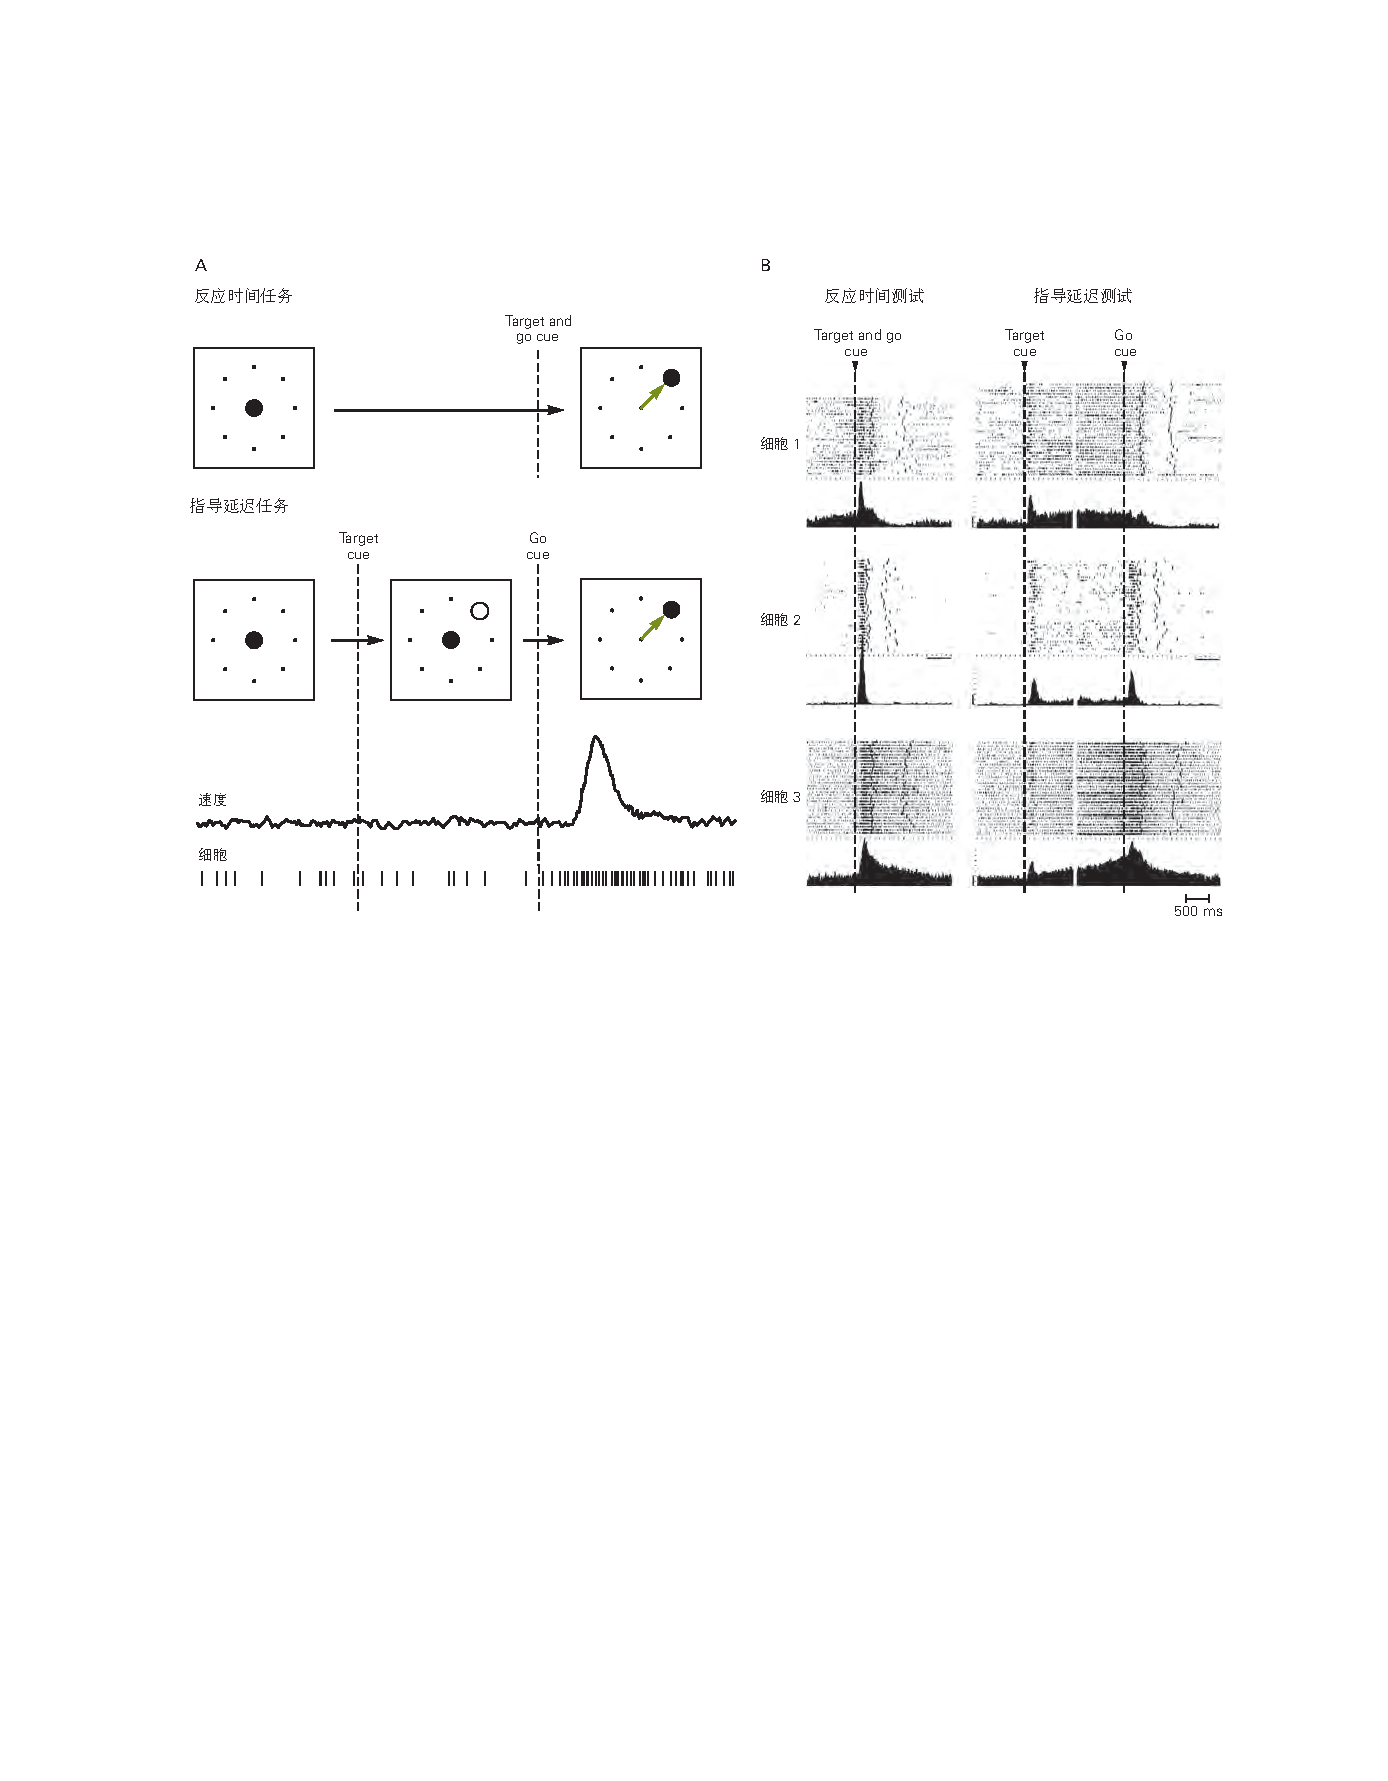
\includegraphics[width=1.0\linewidth]{chap34/fig_34_4}
	\caption*{与运动规划和运动执行相关的神经过程可以及时分离。 (经许可转载自 Crammond 和 Kalaska 2000。)
	A. 在反应时间任务中,感官提示指示受试者移动到哪里(目标提示)和何时移动(去提示)。 计划和启动运动执行所需的所有神经操作都在提示出现和运动开始之间的短暂时间内执行。 在指示性延迟任务中,初始提示告诉受试者移动到哪里,然后才给出开始提示。 第一个提示提供的知识允许主体计划即将到来的动作。 在第一个提示之后但在第二个提示之前发生的任何活动变化都被认为是计划阶段的神经相关因素。
	B. 运动计划和执行在给定皮层区域的单个神经元或神经群水平上并未完全分离。 光栅图和累积直方图显示三个前运动皮层神经元在反应时间试验和指示延迟试验期间对每个细胞首选方向运动的反应。 在栅格图中,每一行代表单个试验中的活动。 每个光栅行中的细抽动表示动作电位,两个较粗的抽动表示运动的开始和结束。 在反应时间试验中,猴子在目标出现之前不知道向哪个方向移动。 相比之下,在指示延迟试验中,初始提示会在第二个信号出现之前通知猴子目标所在的位置,以启动运动。 在延迟期间,许多运动前细胞的活动显示出定向调整的变化,表明即将发生的延迟运动的方向。 单元格 1 中的活动似乎与任务的计划阶段密切相关,因为在指示延迟任务中,在发出信号后没有执行相关的活动。 其他两个单元格显示与计划和执行相关的不同程度的活动。}
\end{figure}


\section{顶叶皮层提供有关世界和身体的信息,用于状态估计以计划和执行电机动作}
感官信息对于选择适当和有效的行动至关重要。 在从杯子喝水之前,大脑会使用视觉输入来识别哪个物体是杯子,它相对于身体的位置,以及它的物理特性,如大小、形状和手柄方向。 此外,有关手臂和手的当前姿势和运动的信息是通过将来自肢体的本体感受信号与运动命令的效应副本相结合来提供的(第 30 章)。 最后,皮肤信号在与物体进行手动交互时至关重要,例如抓住和举起杯子。

几行证据表明顶叶皮层是运动动作感觉处理中的关键大脑区域。 顶叶,尤其是 PE、PEip 和 MIP,从 S-I 接收关于身体姿势和运动的强烈躯体感觉输入。 IPS 沿线和 IPS 内的几个顶叶区域是背侧视觉通路的主要组成部分,它处理有关物体的视觉空间信息,这些物体在伸手、抓住和操纵它们时引导手臂和手的运动。 顶叶也与中央前皮质运动区相互连接,为中央前皮质提供运动感觉引导信号,并从相同的中央前区接收运动命令的输出副本。 最后,患有后顶叶皮层病变的人类受试者通常在使用感觉信息指导运动动作时表现出特定的障碍(方框 34-1)。


\subsection{顶叶皮层将感觉信息与运动动作联系起来}
我们将周围的空间体验为一个单一的统一环境,在这个环境中,物体相对于彼此和我们自己都有特定的位置。 经典神经学认为,顶叶通过整合来自不同感觉方式的输入,构建了一个统一的多模态神经表征世界。 这张单一的空间地图被认为提供了空间感知和运动的感官引导所需的所有信息,因此由控制身体不同部位(如眼睛、手臂和身体)的不同运动电路共享。 手。

然而,认为顶叶皮层包含单一地形组织空间表征的想法是不正确的。 相反,后顶叶皮层包含几个不同的功能区域,它们并行工作并接收与不同效应器(例如眼睛、手臂和手)的运动引导相关的感觉和运动输入的不同组合。 这些区域的神经元通常是多模式的,具有视觉和躯体感觉感受野,并且在特定效应器运动之前和运动期间优先放电。 每个功能区域都连接到参与控制相同效应器的额叶运动区域。 最后,每个区域都不是按照熟悉的周围空间的忠实点对点表示的拓扑结构组织的,而是包含具有不同感觉输入的神经元的复杂混合物,这些神经元可能有助于引导运动动作所需的多感觉整合 环境。



\subsection{身体位置和运动在后顶叶皮层的几个区域表示}
S-I 和相邻的上顶叶皮层区域 PE、MIP 和 PEip 是关于身体部位的位置和运动的本体感受和触觉感觉信息的主要来源。 S-I 区域 1 和 2 中的神经元通常对来自对侧身体有限部分的触觉输入或一个或几个相邻关节在特定方向上的运动做出反应。

相反,许多 PE 和 MIP 神经元在多个关节的被动和主动运动期间放电。 一些细胞也会在多个身体部位的联合运动中做出反应,包括双臂的双边运动。 许多 PE 和 MIP 神经元也有较大的触觉感受野,其反应受肢体运动或姿势期间的情境调节。 例如,具有覆盖手的整个无毛(手掌)表面的触觉感受野的神经元可能仅在手靠近身体时才对与物体的物理接触做出反应,而不是当它用手臂完全接触物体时 扩展。

这些发现表明,虽然区域 1 和区域 2 神经元对特定身体部位的位置和运动进行编码,但上顶叶神经元整合了有关各个关节位置以及肢体节段相对于身体的位置的信息。 这种集成创建了一个神经“身体图式”,它提供了关于手臂相对于身体的位置以及不同的手臂部分如何相对于彼此定位和移动的信息。 这种身体模式对于选择如何实现行为目标和持续控制运动至关重要。

例如,有效伸手的关键要求是了解手臂在伸手之前和期间的位置。 在 Brodmann 区 2 和邻近的上顶叶小叶(区域 5 或 PE)有实验性损伤的猴子在没有视觉的情况下,在本体感受和触觉引导下,无法触及和操纵物体。 具有类似病变的人类患者表现出相同的缺陷,没有空间忽视,这是下顶叶更多横向病变的常见结果。


\subsection{空间目标在后顶叶皮层的几个区域都有体现}
IPS 内的功能区域与空间信息的处理密切相关,尤其是与行动相关的视觉信息。 这些区域中的每一个都有独特的方式来表示相对于身体的物体和空间目标,并有助于控制身体不同部位的运动动作。 例如,外侧顶内区域 (LIP) 中的许多神经元接收来自纹状体皮质区域的视觉输入。 它们的感受野固定在视网膜坐标中,并在猴子改变注视方向时转移到新的空间位置。 当动物注意到感受野内的刺激时,即使不看它,神经反应也常常会增加,并且它们通常会在针对它们感受野中的视觉刺激的眼跳之前放电(图 34-5A;参见第 1 章) 35).

几个顶叶区域优先参与手臂和手部运动的控制。 例如,上顶叶皮层的最内侧区域 V6A 和 PEc 区域接收来自纹状体外视觉区域 V2 和 V3 的输入。 许多 V6A 和 PEc 神经元在视网膜坐标中具有视觉感受野,但它们的活动也经常受到注视方向、当前手臂姿势和伸手动作方向的调节。

IPS 底部的腹侧顶内区 (VIP) 接收来自背侧视觉流的两个组成部分的输入,即内侧颞叶皮层和内侧颞上皮层,它们参与光流和视觉运动的分析。 许多 VIP 神经元对视觉刺激和体感刺激做出反应,其感受野位于面部或头部,在某些情况下,还位于手臂或躯干上。 神经活动处于以头部为中心的坐标中,因为即使眼睛移动以注视不同的空间位置,体感和视觉信息仍保持在记录中(图 34-5B)。 一些 VIP 神经元对沿同一方向移动的视觉和触觉刺激都有反应,而其他神经元则被向其触觉感受野移动的视觉刺激强烈激活,但前提是运动路径最终会与触觉感受野相交。 这些神经元可以让猴子将物体在他们直接的周围空间中的位置和运动与他们身体的不同部位联系起来。

与到达相关的顶叶皮层的另一个区域是顶叶到达区域 (PRR)。 PRR 可能对应于内侧顶内皮层 (MIP) 和相邻的上顶叶皮层和下顶叶皮层的臂控制部分。 许多 PRR 神经元的活动随着到达目标相对于手的位置而变化。 然而,此信号并未固定在手或目标的当前位置,而是固定在当前注视方向(图 34-5C)。 每次猴子朝不同的方向看时,PRR 神经元的触及相关活动都会发生变化,即使目标和手的位置以及所需的触及轨迹没有改变。 相比之下,PE 和 PEip 区域中许多神经元的触及相关活动与注视的相关性较低,而与当前手部位置和手臂姿势的相关性更强。 与 PRR 相比,PE 和 PEip 神经元因此提供了关于相对于手的当前位置的到达目标位置的更稳定的信号。

最后,前顶内区 (AIP) 中的神经元主要涉及通过手的运动来抓取和操纵物体。 许多 AIP 神经元在伸手去拿和抓住特定形状、大小和空间方向的物体时优先活跃,甚至经常在抓住它们之前查看这些物体时(图 34-5D)。 神经反应特性范围很广,从几乎只对物体的视觉输入做出反应但对抓取动作没有反应的神经元,到即使在黑暗中也只在手部运动时放电的神经元。 这表明 AIP 包含神经回路,这些神经回路开始将有关物体物理特性的视觉信息(与处理方式相关)——詹姆斯·吉布森 (James Gibson) 称之为物体的可供性——转化为适当的手部动作(第 56 章)。

关于顶叶皮层的一个有趣发现是,神经元的感受野可以通过个人经历(例如工具使用)而改变。 训练猴子使用耙形工具取回手臂和手正常够不到的食物颗粒。 许多 VIP 神经元通常会对位于手的当前位置附近或手臂可触及的任何地方的视觉对象做出反应。 训练后,当猴子抓住工具时,它们的视觉感受野会瞬时扩大以吸收工具,就好像工具的远端已经成为猴子自己手和手臂的功能延伸(图 34-6)。


\subsection{内部产生的反馈可能影响顶叶皮层活动}
将手臂运动的视觉和躯体反馈从外周传递到皮层回路的延迟会导致实时感觉运动控制的振荡甚至不稳定。 这个问题的一个理论解决方案是使用前向内部模型,根据传出运动命令的内部效应副本以及较慢的外围反馈信号(第 30 章)对身体运动进行预测估计。

几行证据表明,顶叶皮层回路和小脑(第 37 章)可能实现类似的解决方案。 PE、MIP 和 PRR 中的许多与到达相关的神经元不仅在响应被动感觉输入时活跃,而且在运动开始之前和延迟到达任务的指示延迟期间也是活跃的。 这些反应表明这些神经元在运动开始之前处理集中生成的关于运动意图的信号。 这种运动前活动通常被解释为顶叶皮层产生有助于早期运动规划的前馈信号的证据。 然而,另一种解释是运动前活动是由预期运动的运动命令的输出副本驱动的,该运动命令通过与中央前运动区域的相互连接传输到顶叶皮层。 这种外周感觉输入和中央效应副本的组合可以允许一些与顶叶触及相关的电路计算对手臂当前状态及其相对于行为目标的位置的持续更新估计。 该估计可用于快速纠正正在进行的手臂运动中的错误。

顶叶回路是主要参与受试者运动意图的形成还是状态估计将取决于其运动前活动的起源。 如果它主要在顶叶皮层本身内产生,这将强烈暗示顶叶皮层参与了预期运动的规划。 相比之下,如果它主要由从中央前运动区域中继的输出副本驱动,这将强烈暗示顶叶回路参与状态估计,包括预测手臂应如何响应运动命令而移动。



\section{前运动皮层支持运动选择和规划}
\subsection{内侧前运动皮层参与自主行为的情境控制}
\subsection{背侧前运动皮层参与规划手臂的感觉引导运动}
\subsection{背侧前运动皮层参与应用管理行为的规则(关联)}
\subsection{腹侧前运动皮层参与规划手的运动动作}
\subsection{前运动皮层可能有助于指导运动行为的知觉决策}
\subsection{当观察到其他人的运动动作时,几个皮层运动区会活跃}
\subsection{自主控制的许多方面分布在顶叶和前运动皮层}

\section{初级运动皮层在运动执行中起着重要作用}
\subsection{初级运动皮层包括运动外围的详细地图}
\subsection{初级运动皮层中的一些神经元直接投射到脊髓运动神经元}
\subsection{初级运动皮层的活动反映了运动输出的许多时空特征}
\subsection{初级运动皮层活动也反映了运动的高阶特征}
\subsection{感觉反馈迅速传递到初级运动皮层和其他皮层区域}
\subsection{初级运动皮层是动态的和适应性强的}

\section{要点}
\subsection{荐读}
\subsection{参考文献}